%!TEX TS-program = xelatex

% HSE Beamer Theme
% by Danil Fedorovykh
% http://hse.ru/staff/df
%
% Version 2.0 (English)
% January 2022

%%% Set up the free HSE Sans font
%%% https://www.hse.ru/info/brandbook/#font

\documentclass[aspectratio=169]{beamer}

\newbool{russian}
\booltrue{russian} % Uncomment if in Russian
\usepackage{HSE-theme/beamerthemeHSE} % Load HSE theme
\usepackage[no-math]{fontspec}      % fonts loading
\usepackage{caption}
\usepackage{subfigure}
\usepackage{subcaption}
\usepackage{hyperref}
\usepackage[dvipsnames]{xcolor}
\usepackage{ragged2e}
\captionsetup[figure]{labelformat=empty}
\captionsetup[subfigure]{labelformat=empty}
\renewcommand*{\thesubfigure}{(\arabic{subfigure})}
\setsansfont{HSE Sans}
%\graphicspath{{./images/}}
\graphicspath{{/home/llyy/Yandex.Disk/personal/knowledge/general/algorithms_course/repo/algorithms_course/4_search/lection/images}}


%%% Информация об авторе и выступлении
\title[Title]{Алгоритмы и структуры данных} 
\subtitle{Лекция 4. Алгоритмы поиска}
\author[Author's name]{Илья Сергеевич Бычков\\ \smallskip \scriptsize \url{ibychkov@hse.ru}}
\institute{НИУ ВШЭ - Нижний Новгород}
\date{\today}


\begin{document}

\frame[plain]{\titlepage}

%%%%%%%%%%%%%%%%%%%%%%%%%%%%%%%%%%%%%%%%%%%%%%%%%%%%%%%%%%%%%%%%%%%%%%%%%%%%%%%%%%%%%%%%%%%%%%%%%%
\begin{frame}[c]
%\frametitle{A first slide}

\begin{center}
\Huge Лекция 4.

\Huge Алгоритмы поиска
\end{center}

\end{frame}

%%%%%%%%%%%%%%%%%%%%%%%%%%%%%%%%%%%%%%%%%%%%%%%%%%%%%%%%%%%%%%%%%%%%%%%%%%%%%%%%%%%%%%%%%%%%%%%%%%
\begin{frame}
\frametitle{Алгоритмы поиска}
\framesubtitle{План лекции}

\begin{enumerate}
  \setcounter{enumi}{-1}
  \item{План лекции}
  \item{\textcolor{blue}{Задача поиска}}
  \item{Линейный поиск}
  \item{Двоичный/бинарный поиск}
  \item{Троичный/тернарный поиск}
  \item{Экспоненциальный поиск}
  \item{Jump поиск}
\end{enumerate}
\end{frame}



%%%%%%%%%%%%%%%%%%%%%%%%%%%%%%%%%%%%%%%%%%%%%%%%%%%%%%%%%%%%%%%%%%%%%%%%%%%%%%%%%%%%%%%%%%%%%%%%%%
\begin{frame}
\frametitle{Задача поиска}
\framesubtitle{Задача поиска}
\justifying
\textcolor{red}{Задача поиска} заключается в нахождении объектов с заданными свойствами среди конечного количества объектов.
\newline\newline
\textcolor{blue}{Входные данные}: коллекция/контейнер с объектами, искомый критерий \newline (функция/предикат)\newline\newline
\textcolor{blue}{Выходные данные}: информация о местоположении искомых объектов в коллекции (обычно индекс или набор индексов)\newline\newline
Задача поиска является самой фундаментальной задачей в области компьютерных наук.
\end{frame}


%%%%%%%%%%%%%%%%%%%%%%%%%%%%%%%%%%%%%%%%%%%%%%%%%%%%%%%%%%%%%%%%%%%%%%%%%%%%%%%%%%%%%%%%%%%%%%%%%%
\begin{frame}
\frametitle{Алгоритмы поиска}
\framesubtitle{План лекции}

\begin{enumerate}
  \setcounter{enumi}{-1}
  \item{План лекции}
  \item{Задача поиска}
  \item{\textcolor{blue}{Линейный поиск}}
  \item{Двоичный/бинарный поиск}
  \item{Троичный/тернарный поиск}
  \item{Экспоненциальный поиск}
  \item{Jump поиск}
\end{enumerate}
\end{frame}


%%%%%%%%%%%%%%%%%%%%%%%%%%%%%%%%%%%%%%%%%%%%%%%%%%%%%%%%%%%%%%%%%%%%%%%%%%%%%%%%%%%%%%%%%%%%%%%%%%
\begin{frame}
\frametitle{Линейный поиск}
\framesubtitle{Линейный поиск}
\justifying
\textcolor{red}{Линейный поиск (linear search)} — простейший алгоритм поиска (полный перебор).\newline\newline Заключается в последовательной проверке каждого элемента коллекции на \newline соответствие заданному критерию поиска. \newline\newline Алгоритм выполняется пока не будет найдено совпадение(или все совпадения) или не будут проверены все элементы.

\begin{figure}
    \captionsetup[subfigure]{labelformat=empty}
    \centering
    \subfigure[{ \scriptsize Линейный поиск (linear search), Источник - \href{https://www.geeksforgeeks.org/linear-search/}{Geeks4Geeks}}]{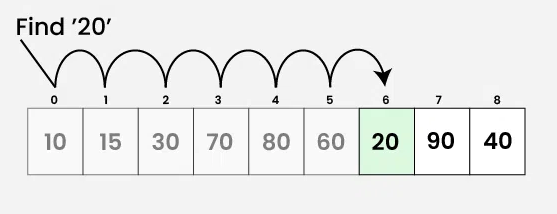
\includegraphics[width=75mm, height=28mm]{linear_search}} 
\end{figure}
\end{frame}

%%%%%%%%%%%%%%%%%%%%%%%%%%%%%%%%%%%%%%%%%%%%%%%%%%%%%%%%%%%%%%%%%%%%%%%%%%%%%%%%%%%%%%%%%%%%%%%%%%
\begin{frame}
\frametitle{Линейный поиск}
\framesubtitle{Линейный поиск}
\justifying
\textcolor{red}{Линейный поиск (linear search)} \newline\newline
Преимущества:\newline
\textcolor{green} {\textbf{+}} крайне прост в реализации\newline
\textcolor{green} {\textbf{+}} может работать без какой-либо дополнительной информации о данных\newline\newline
Недостатки:\newline
\textcolor{red} {\textbf{-}} линейная сложность $\mathcal{O}(n)$ по времени в худшем и среднем случаях\newline

Алгоритм использует константный размер дополнительной памяти $\mathcal{O}(1)$. \newline Однако, это является общим свойством для большинства алгоритмов поиска.
\end{frame}

%%%%%%%%%%%%%%%%%%%%%%%%%%%%%%%%%%%%%%%%%%%%%%%%%%%%%%%%%%%%%%%%%%%%%%%%%%%%%%%%%%%%%%%%%%%%%%%%%%
\begin{frame}
\frametitle{Алгоритмы поиска}
\framesubtitle{План лекции}

\begin{enumerate}
  \setcounter{enumi}{-1}
  \item{План лекции}
  \item{Задача поиска}
  \item{Линейный поиск}
  \item{\textcolor{blue}{Двоичный/бинарный поиск}}
  \item{Троичный/тернарный поиск}
  \item{Экспоненциальный поиск}
  \item{Jump поиск}
\end{enumerate}
\end{frame}

%%%%%%%%%%%%%%%%%%%%%%%%%%%%%%%%%%%%%%%%%%%%%%%%%%%%%%%%%%%%%%%%%%%%%%%%%%%%%%%%%%%%%%%%%%%%%%%%%%
\begin{frame}
\frametitle{Двоичный (бинарный) поиск}
\framesubtitle{Двоичный (бинарный) поиск}
\justifying
\textcolor{red}{Двоичный/бинарный поиск (binary search)} — классический алгоритм поиска элемента в \textcolor{blue}{отсортированном} массиве (векторе).\newline\newline Делит текущий рассматриваемый интервал альтернатив пополам. В зависимости от значения элемента в середине интервала рекурсивно решает такую же подзадачу для левой половины или для правой.


\begin{figure}
    \captionsetup[subfigure]{labelformat=empty}
    \centering
    \subfigure[{ \scriptsize Линейный поиск (linear search), Источник - \href{https://www.geeksforgeeks.org/linear-search/}{Geeks4Geeks}}]{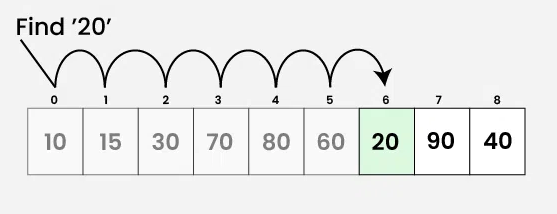
\includegraphics[width=75mm, height=28mm]{linear_search}} 
\end{figure}
\end{frame}

\end{document}